% THIS IS SIGPROC-SP.TEX - VERSION 3.1
% WORKS WITH V3.2SP OF ACM_PROC_ARTICLE-SP.CLS
% APRIL 2009
%
% It is an example file showing how to use the 'acm_proc_article-sp.cls' V3.2SP
% LaTeX2e document class file for Conference Proceedings submissions.
% ----------------------------------------------------------------------------------------------------------------
% This .tex file (and associated .cls V3.2SP) *DOES NOT* produce:
%       1) The Permission Statement
%       2) The Conference (location) Info information
%       3) The Copyright Line with ACM data
%       4) Page numbering
% ---------------------------------------------------------------------------------------------------------------
% It is an example which *does* use the .bib file (from which the .bbl file
% is produced).
% REMEMBER HOWEVER: After having produced the .bbl file,
% and prior to final submission,
% you need to 'insert'  your .bbl file into your source .tex file so as to provide
% ONE 'self-contained' source file.
%
% Questions regarding SIGS should be sent to
% Adrienne Griscti ---> griscti@acm.org
%
% Questions/suggestions regarding the guidelines, .tex and .cls files, etc. to
% Gerald Murray ---> murray@hq.acm.org
%
% For tracking purposes - this is V3.1SP - APRIL 2009

\documentclass{acm_proc_article-sp}

\usepackage{caption}
\usepackage{soul}
\usepackage{color}
\usepackage{url}
\usepackage{hyperref}
\usepackage{subfig}
\usepackage{graphicx}
\usepackage{algpseudocode}

\begin{document}
\title{Determining RNA Secondary Structure}
\subtitle{Assignment 5}
%
% You need the command \numberofauthors to handle the 'placement
% and alignment' of the authors beneath the title.
%
% For aesthetic reasons, we recommend 'three authors at a time'
% i.e. three 'name/affiliation blocks' be placed beneath the title.
%
% NOTE: You are NOT restricted in how many 'rows' of
% "name/affiliations" may appear. We just ask that you restrict
% the number of 'columns' to three.
%
% Because of the available 'opening page real-estate'
% we ask you to refrain from putting more than six authors
% (two rows with three columns) beneath the article title.
% More than six makes the first-page appear very cluttered indeed.
%
% Use the \alignauthor commands to handle the names
% and affiliations for an 'aesthetic maximum' of six authors.
% Add names, affiliations, addresses for
% the seventh etc. author(s) as the argument for the
% \additionalauthors command.
% These 'additional authors' will be output/set for you
% without further effort on your part as the last section in
% the body of your article BEFORE References or any Appendices.

%\numberofauthors{3} %  in this sample file, there are a *total*
% of EIGHT authors. SIX appear on the 'first-page' (for formatting
% reasons) and the remaining two appear in the \additionalauthors section.
%
\numberofauthors{1}
\author{
	\alignauthor Caitlin Ross\\
	\affaddr{Computer Science Department, Rensselaer Polytechnic Institute} \\
	\email{rossc3@rpi.edu}
}
% There's nothing stopping you putting the seventh, eighth, etc.
% author on the opening page (as the 'third row') but we ask,
% for aesthetic reasons that you place these 'additional authors'
% in the \additional authors block, viz.

\date{30 July 1999}
% Just remember to make sure that the TOTAL number of authors
% is the number that will appear on the first page PLUS the
% number that will appear in the \additionalauthors section.

\maketitle

\begin{abstract}
This work predicts the RNA secondary structure of multiple RNA sequences that code for prions.  First MUSCLE is used to get the alignment sequences.  Then the aligned sequences are used in a comparative sequence analysis to predict the secondary structure of the consensus sequence.  The program developed here outputs the consensus sequence, along with the secondary structure in dot-bracket notation.  This information can then be used as input into a third party tool that plots the secondary structure.  
\end{abstract}


\section{Problem Statement}
The problem here is to take multiple RNA sequences and predict the secondary structure.  The RNA sequences given are genes that code for prions.  RNA secondary structure is important because this structure tends to be more conserved than the actually RNA sequence.  Thus the secondary structure is more important than actual sequence in understanding the function of the RNA.  

\section{Methods}
We were given 42 RNA sequences in the PRP.fa fasta file.  First we use the MUSCLE mutli-sequence aligner to align the sequences.  This results in 42 alignments that are 42 bases long.  Then we wrote a Python program to determine the secondary structure from the RNA alignments.  After reading in the alignments with BioPython, the consensus sequence for the alignments is found.  The consensus sequence is found by counting each symbol $b \in \{A, C, G, U, -\}$ in each column and taking the symbol with the most occurrences in each column.  

Next we use comparative sequence analysis for the RNA secondary structure prediction.  For this, we must first calculate the mutual information matrix, which looks at pairwise joint frequencies in the alignments.  The mutual information matrix $M$ is an $L \times L$ matrix, where $L$ is the number of columns in the alignments.  Then for aligned columns $i$ and $j$, we have 
\begin{equation} M_{ij} = \sum_{x_i,x_j} f_{x_ix_j} \log_2 \frac{f_{x_ix_j}}{f_{x_i}f_{x_j}}, \end{equation}
where $x_i,x_j \in \{A, C, G, U\}$ for columns $i$ and $j$, respectively.  $f_{x_i}$ is the frequency of the base $x_i$ observed in column $i$, whereas $f_{x_ix_j}$ is the pairwise frequency of one of the possible base pairs observed in columns $i$ and $j$.  For this, we only consider the base pairs AU, UA, CG, GC, GU, and UG to be valid base pairs for the calculation of $M_{ij}$.  For all other base pairs, $f_{x_ix_j} = 0$.  In the case where any frequencies in equation (1) are 0, we set $\log_2 \frac{f_{x_ix_j}}{f_{x_i}f_{x_j}} = 0$.  For any $M_{ij} < 0$, we set $M_{ij} = 0$.

Now we use dynamic programming to calculate the maximum mutual information secondary structure from $M_{ij}$.  For this, we define a matrix $D$, which is also an $L \times L$ matrix.  We start by initializing $D_{ij} = 0,  \forall i,j \in L$.  Then $D$ is calculated by the following algorithm (note that we assume a starting 0-index).  The end result is $D$, which is an upper triangular matrix.
\begin{algorithmic}
\For{i = L -1..0} 
	\For{ j = i+3..L} \\
		 \State $D(i,j) = max\left\{
		\begin{array}{ll}
		D(i+1,j) \\
		D(i, j-1) \\
		D(i+1,j-1) + M_{ij} \\
		max_{i<k<j}[D(i,k) + D(k+1, j)]
		\end{array}
		\right.$
	\EndFor
\EndFor
\end{algorithmic}
  
At this point, we use a back trace algorithm to trace through matrix $D$ to find the base pairs for the RNA secondary structure.  The code for the BackTrace algorithm given in the nussinov.py program on the course webpage was used here. The BackTrace() function uses the original mutual information matrix, $M_{ij}$, the matrix $D$, and the consensus sequence found earlier to find the pairs.  After getting the list of pairs, the secondary structure can be determined.  Here we find the dot-bracket notation of the secondary structure.  Matching parentheses in positions $i$ and $j$ indicate a base pairing between bases $i$ and $j$, otherwise there is just a dot.  We determine the dot-bracket format using the function StructureFromPairs() from the nussinov.py program, which takes in the pairs found previously.  

Now the secondary structure can be plotted from the dot-bracket notation.  We use the website \\ http://nibiru.tbi.univie.ac.at/forna/ for plotting.  We provide the consensus sequence with the dot-bracket notation.  

\begin{figure}[!b]
	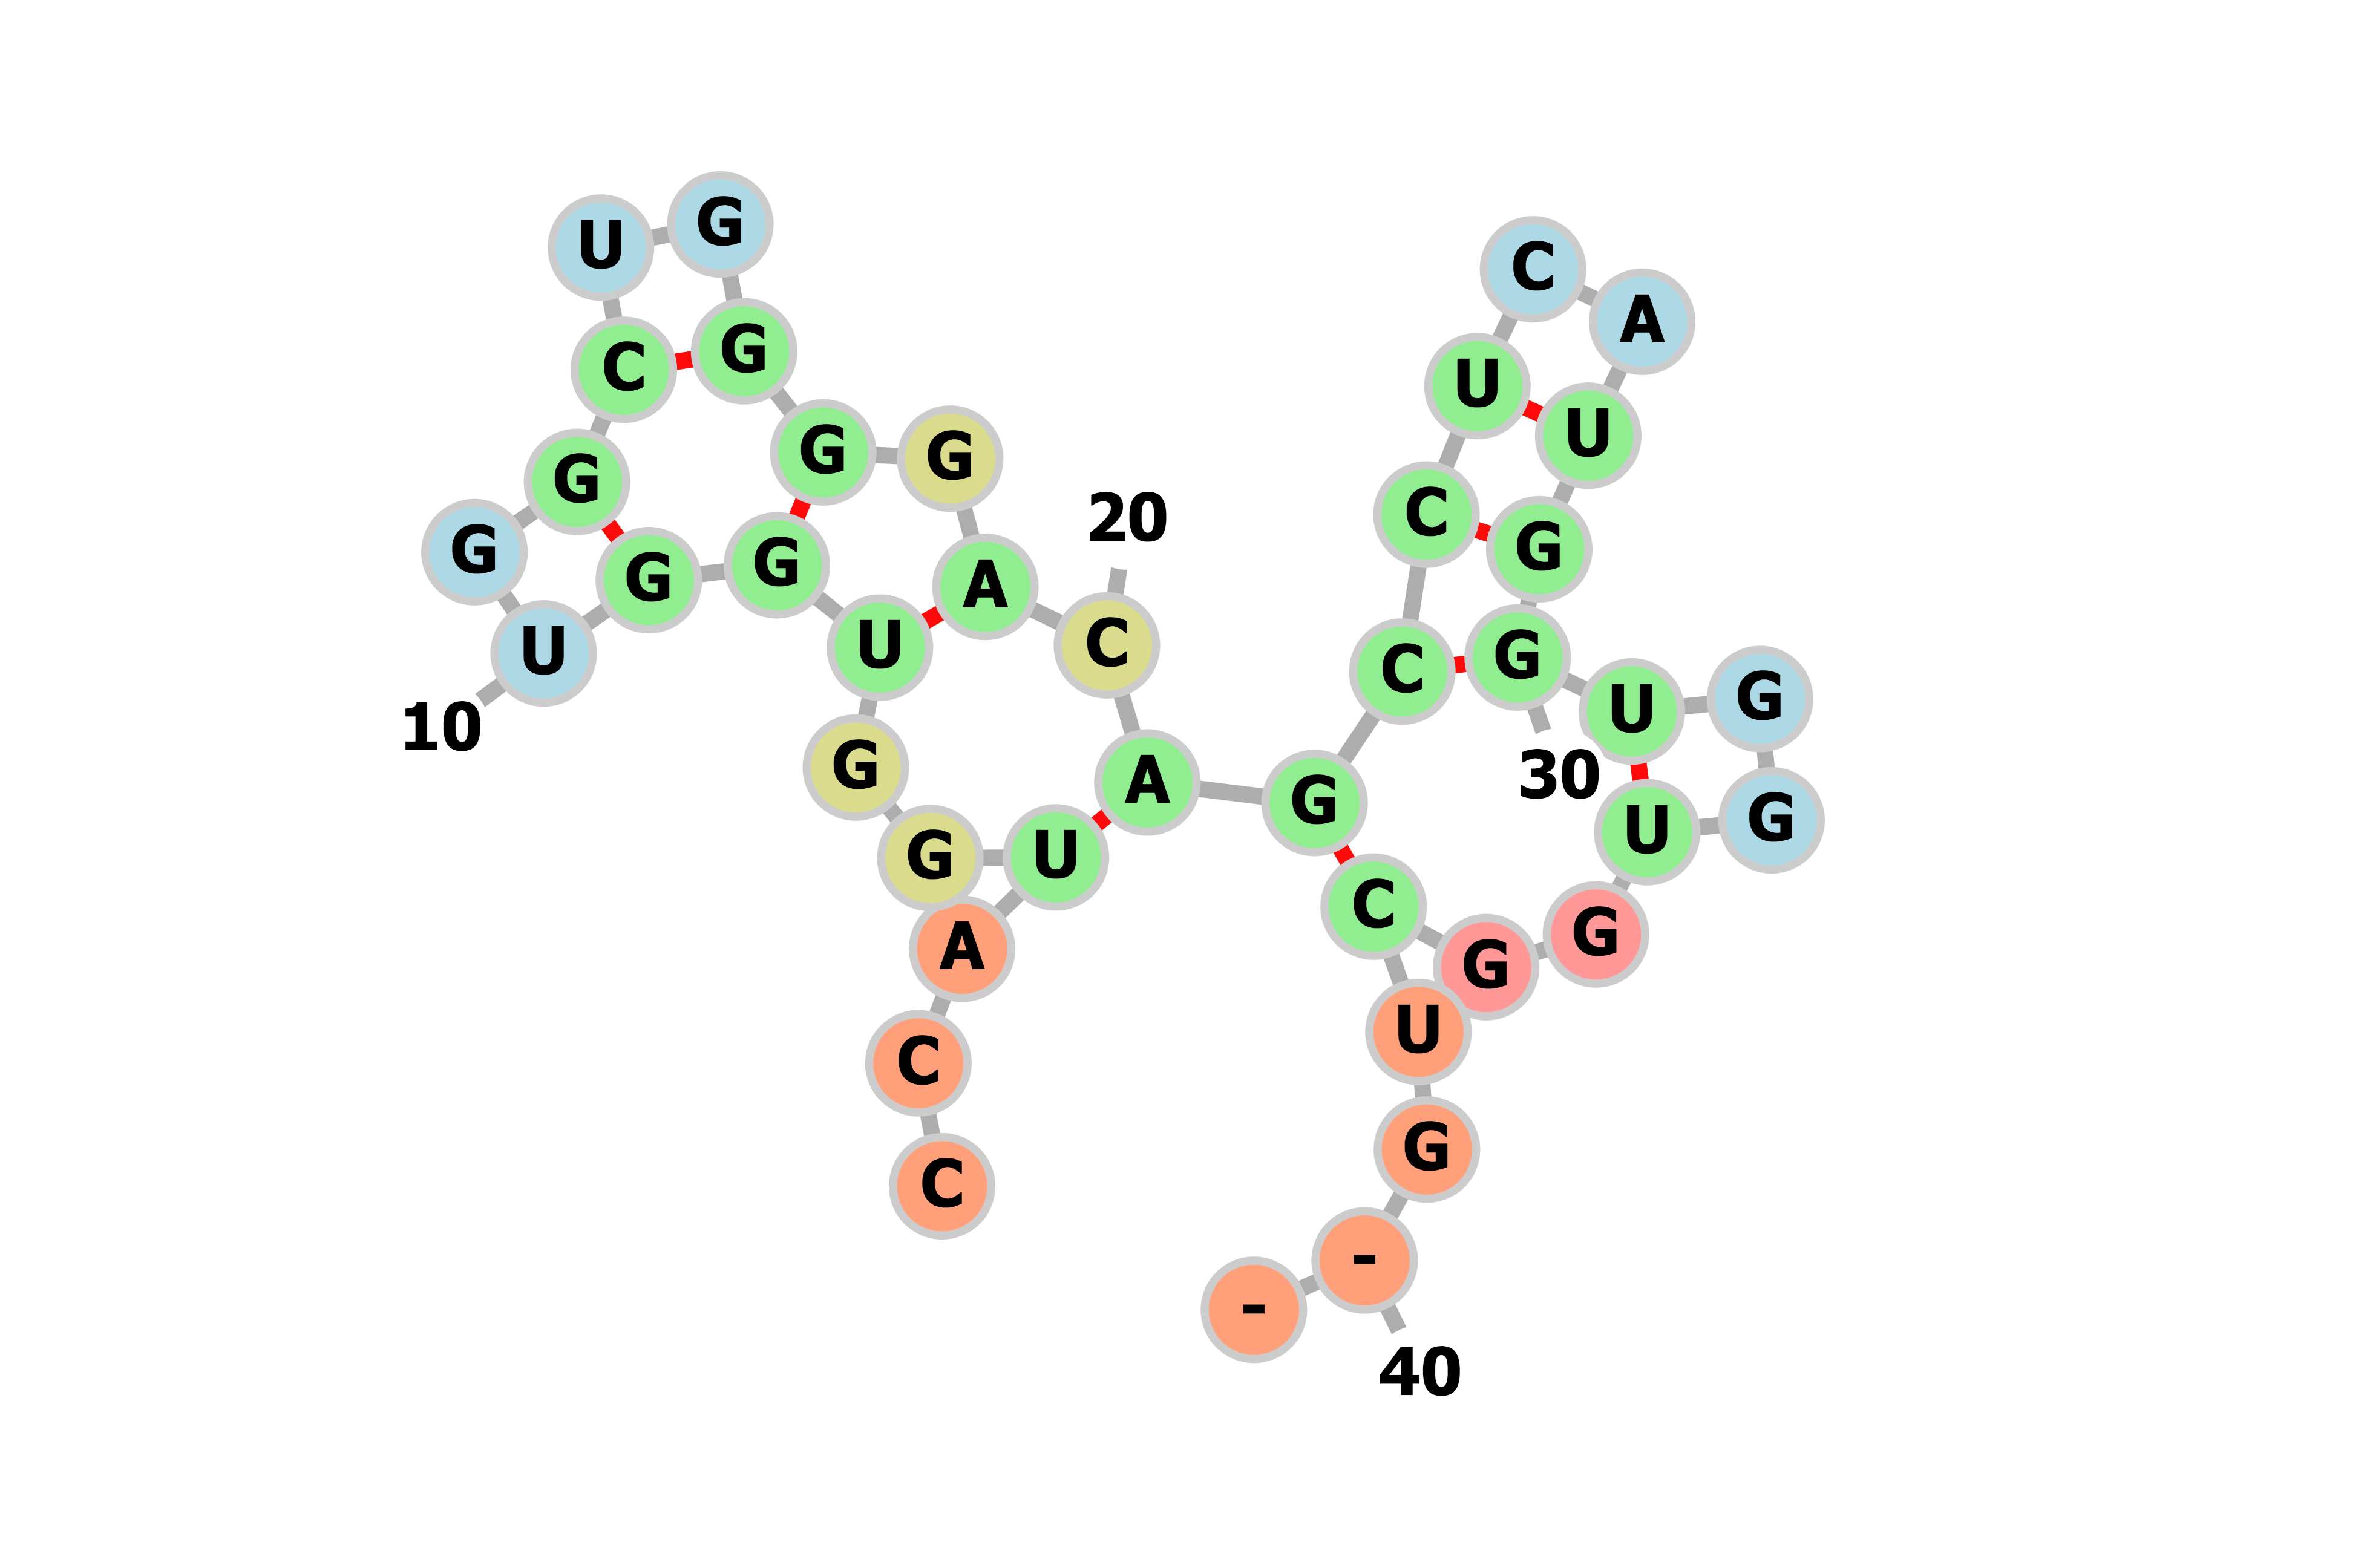
\includegraphics[trim={0 0 2cm 0}, clip,width=3.5in]{rna.png}
	\caption{Plotted RNA secondary structure for the consensus sequence.}
	\label{fig:hist}
\end{figure}

\section{Results}
The consensus sequence found by the program is \\ CCAUGGUGGUGGCUGGGGACAGCCUCAUGGUGGU\\GGCUG--.  The secondary structure found, in dot-bracket notation, is '...(..(((..)(..)).).)((((..)))(..)..).....'.  Figure 1 shows the RNA secondary structure plotted.  Red lines show the base pairs.  




%
% The following two commands are all you need in the
% initial runs of your .tex file to
% produce the bibliography for the citations in your paper.
\bibliographystyle{abbrv}
%\bibliography{sigproc}  % sigproc.bib is the name of the Bibliography in this case

% You must have a proper ".bib" file
%  and remember to run:
% latex bibtex latex latex
% to resolve all references
%
% ACM needs 'a single self-contained file'!
%
%APPENDICES are optional
%\balancecolumns

\balancecolumns
% That's all folks!
\end{document}
